\section{System overview and management model}
\label{sec:system}

HMRS is a self-hosted knowledge document management system for converting
heterogeneous documents into managed, searchable collections. A Python
parsing service, a TypeScript web application and an MCP tool server share
local storage and retrieval engines \cite{mcp}. The design follows from the
dependency chain of Section~\ref{sec:intro}: what a document is parsed as
determines what can be indexed, the collection it is filed into determines
which tier can see it, and the tiers that follow determine whether a
supporting passage is ever read. The primary object of the design is therefore
the managed collection rather than the query. State is made auditable through
three sources---the document files, the tree registry and per-library
metadata---so that a management operation can be checked against what it
claimed to do. Each check belongs to the platform operation or calling
workflow that performs it, and the evaluation reports evidence at that level.

\subsection{Management levels and the tiered access path}
\label{sec:levels}

The access path has four views over three managed object levels. The catalogue
view exposes collections and their descriptions; the shelf view exposes
(document, description) entries within a selected collection; the document view
opens a document body; and the segment view exposes indexed parts and, when
invoked, their evidence scores and provenance. The shelf is a listing view, not
a fourth storage level, and a pinned search may bypass catalogue and shelf
selection. The levels describe maintained objects and operations; the views
describe what a query or agent can inspect and in what order.

\begin{table*}[t]
\centering
\small
\setlength{\tabcolsep}{4pt}
\renewcommand{\arraystretch}{1.15}
\caption{Management levels and the tiered access path. Each level names the
objects it maintains, the operations that write them, the state that describes
them, the tier that reads them, and the measurement that exercises it.
The selected access policy determines which tiers are visited; a pinned
search can bypass catalogue navigation.}
\label{tab:levels}
\begin{tabular}{@{}>{\raggedright\arraybackslash}p{0.12\textwidth}>{\raggedright\arraybackslash}p{0.21\textwidth}>{\raggedright\arraybackslash}p{0.18\textwidth}>{\raggedright\arraybackslash}p{0.12\textwidth}>{\raggedright\arraybackslash}p{0.12\textwidth}>{\raggedright\arraybackslash}p{0.13\textwidth}@{}}
\toprule
Level & Objects and operations & State description & Read tier & Check & Evidence\\
\midrule
Collection & libraries and sub-libraries; automatic assignment from parsed content; description and tag derivation; catalogue listing & library registry, per-library metadata, library-level index & catalogue & catalogue inventory and description round-trip & E1, E2\\
Document & documents and their parts; duplicate review; move, rename, delete; forced re-index & document files, tree registry, per-library metadata & shelf & reconciliation on selected operations & E2\\
Segment & structural split; dense and lexical indices; optional evidence gate & chunk identifiers, per-segment scores with provenance & document and segment & index coverage and post-index probe & E1, E5--E9\\
\bottomrule
\end{tabular}
\end{table*}

At the collection level an ingest agent can classify a parsed document against
the catalogue of library descriptions and select a collection based on its
subject. The same workflow derives descriptions and tags from the body rather
than the filename; these semantic decisions are not enforced by the parse API.
Sub-libraries are first-class tree nodes with their own descriptions and
indices. At the document level, duplicate detection reports candidate pairs for
review rather than deleting them, because adjacent parts may be similar while
carrying distinct sections. Re-indexing remains a separate, explicit operation.
At the segment level a document is split at recognised structural markers and
its parts are indexed for dense and lexical search. When a workflow invokes the
evidence gate, candidate documents are fetched and their segments scored; the
gate returns surviving segments with provenance. This score-based admission
check is distinct from candidate ranking, fusion and workflow-level caps, and
it does not establish that a passage entails an answer claim.

Figure~\ref{fig:levels} shows the management structure alongside an
illustrative catalogue-first access path. This path proceeds as a ladder: the
\emph{catalogue} tier lists collections and their descriptions, the
\emph{shelf} tier lists the documents and their descriptions inside a
selected collection, the \emph{document} tier opens a body, and the
\emph{segment} tier exposes its parts for optional scoring. Figure~\ref{fig:arch} shows the service
boundaries and the shared state these tiers read and write. In a catalogue-first workflow each selection can narrow the scope the next
step considers. Its checks have distinct denominators: a catalogue that does
not contain the owning collection is a different failure from a shelf that
omits the document, and the system reports them separately.

\begin{figure}[t]
\centering
\includegraphics[width=\columnwidth]{fig_analogy_single}
\caption{Library analogy for HMRS management and a catalogue-first access path. The catalogue, shelf and page correspond to collection, document and segment levels; the librarian represents optional evidence judging.}
\label{fig:levels}
\end{figure}

\setcounter{dbltopnumber}{1}
\begin{figure*}[t]
\centering
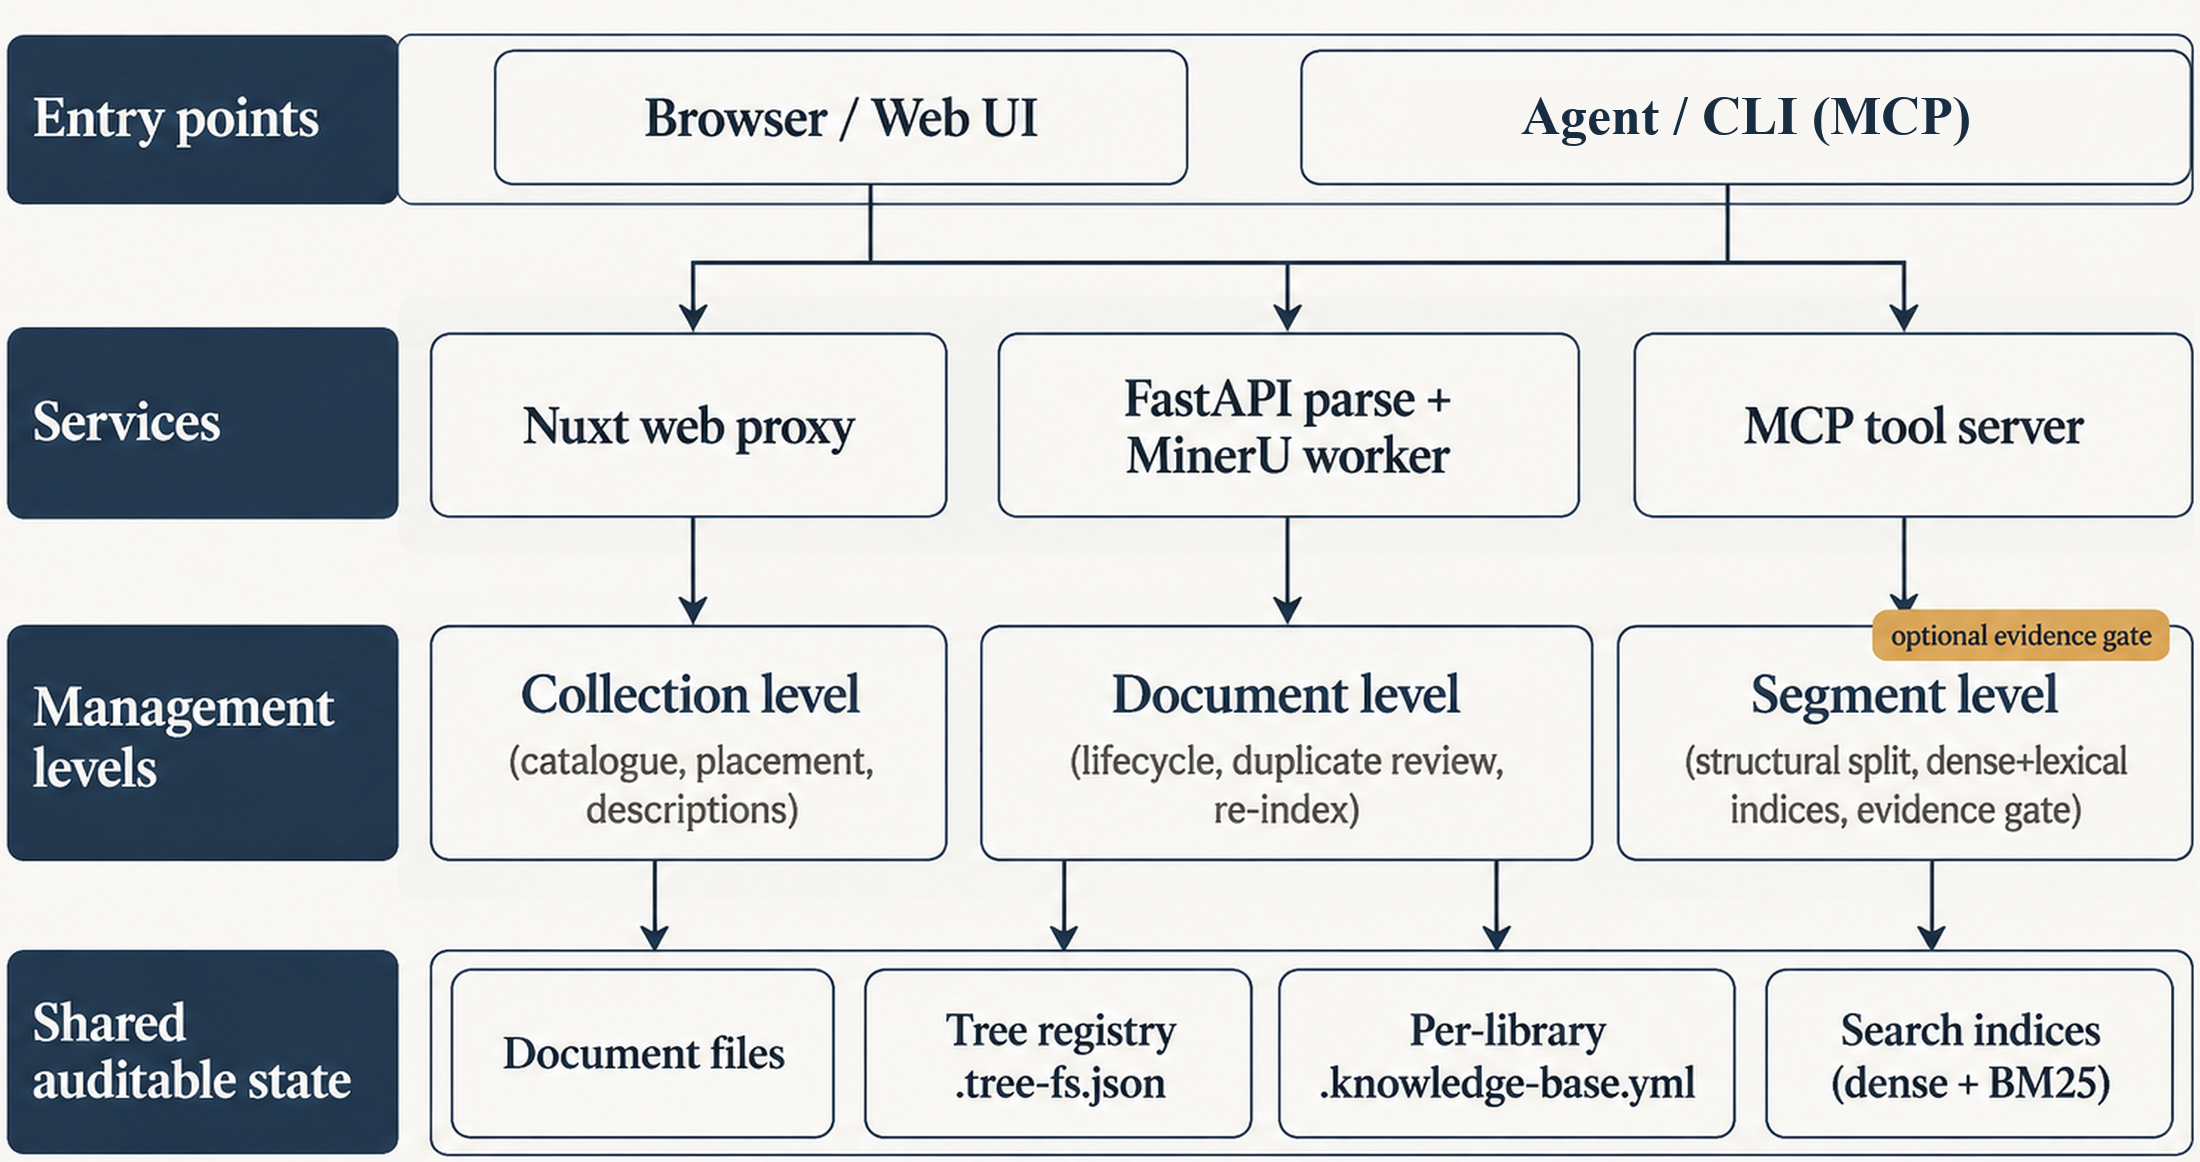
\includegraphics[width=\textwidth]{fig_architecture_cropped}
\caption{HMRS service architecture. Entry points (browser, agent/CLI) reach the Nuxt proxy, the FastAPI+MinerU parse service and the MCP tool server, which operate three management levels over one shared auditable state (document files, tree registry, per-library metadata, search indices). The evidence gate is an optional segment-level call.}
\label{fig:arch}
\end{figure*}

Figure~\ref{fig:workflow} illustrates one query workflow over the managed
collection. The complete system workflow is broader than query serving:
acquisition creates a parsed artefact, organisation assigns it to a collection
and derives descriptions/tags, lifecycle operations update or reconcile its
state, and the access path selects candidate evidence for inspection. The
management path covers acquisition (Section~\ref{sec:acquisition}),
content-informed organisation and lifecycle checks
(Section~\ref{sec:organization}), and the tool and runtime layer
(Section~\ref{sec:implementation}). The chat endpoint defines pinned-search
and all-library librarian policies. Hybrid is a composed retrieval
configuration, not a third built-in server policy; it combines vector and
catalogue calls under an explicit directive. The document graph supports
navigation, not evidence. Experience retrieval and the persona-distillation
workflows reuse knowledge-base infrastructure but follow their own retrieval
and filtering paths; neither is described here as invoking Laya, and neither
was evaluated at scale.

The platform exposes five management domains: acquisition, organisation,
lifecycle, query and operational experience. Some controls are enforced by
API/MCP operations; semantic and quality checks are agent-workflow procedures,
and campaign audits test selected outcomes. Table~\ref{tab:functions}
distinguishes these layers and maps each domain to the evidence that exercises
it.

\begin{table*}[t]
\centering
\small
\setlength{\tabcolsep}{4pt}
\caption{Management functions, the enforcement or workflow check associated
with each, and the evaluation that exercises it. The table separates API/MCP
controls from agent procedures and campaign audits; semantic choices such as
which collection owns a document remain workflow decisions and are measured,
not enforced.}
\label{tab:functions}
\begin{tabular}{@{}>{\raggedright\arraybackslash}p{0.13\textwidth}>{\raggedright\arraybackslash}p{0.37\textwidth}>{\raggedright\arraybackslash}p{0.30\textwidth}>{\raggedright\arraybackslash}p{0.11\textwidth}@{}}
\toprule
Group & Operations & Platform or workflow check & Evidence\\
\midrule
Acquisition & submit, parse (MinerU), quality review, duplicate review, structural split, store, index & parse-task state; workflow quality checks; entry-point-specific deduplication and indexing; post-index probe & E1\\
Organisation & create library or sub-library, content-informed placement, descriptions and tags, duplicate review & API validates identifiers and required fields; workflow checks descriptions and tags; audit compares files, tree and library metadata & E1--E2\\
Lifecycle & move, rename, delete, force re-index, graph build & operation-specific API updates; reconciliation audit detects selected stale or inconsistent state & E2\\
Query & tier selection, vector, keyword, catalogue and two-stage search, gate invocation & endpoint enforces tool allow/deny lists, timeouts and turn limits; invoked gate returns survivor provenance & E5--E9\\
Experience & extract, approve, tier, search & experience tools apply their own retrieval, verification and credibility filters & E4\\
\bottomrule
\end{tabular}
\end{table*}

\begin{figure*}[t]
\centering
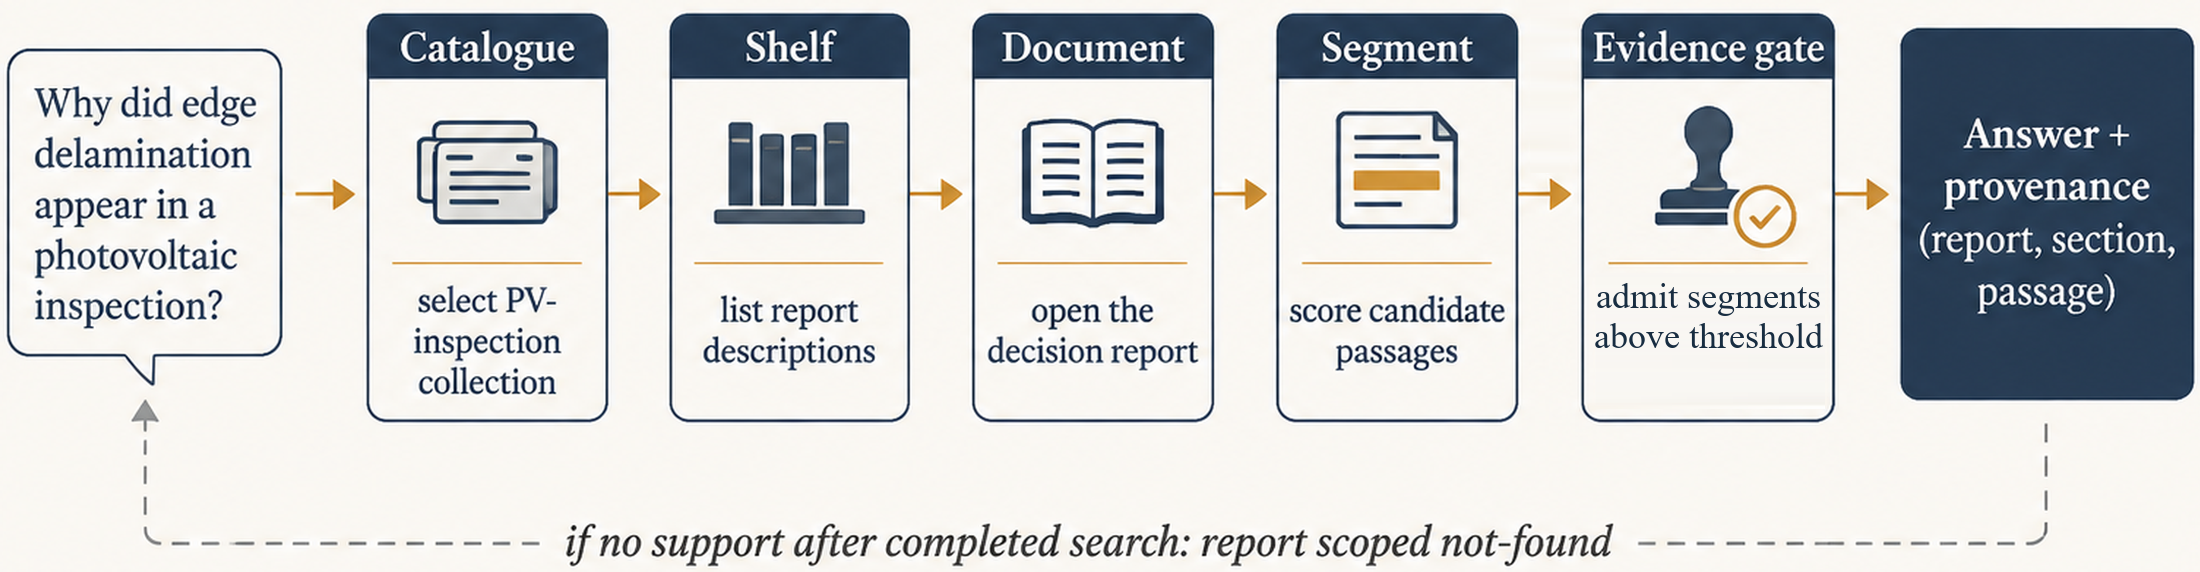
\includegraphics[width=\textwidth]{fig_workflow_demo_cropped}
\caption{Illustrative catalogue-first query path, not an experimental case. A question narrows from catalogue to shelf to document and segment. In the depicted variant, the optional gate admits passages above its score threshold; the agent may then answer with provenance. A completed review without support calls for a scoped not-found report.}
\label{fig:workflow}
\end{figure*}

\subsection{Data model and object lifecycle}
\label{sec:datamodel}
\label{sec:lifecycle}

Documents are Markdown with extracted images. Library state is described by
the document files, the \texttt{.tree-fs.json} registry and each
\texttt{.knowledge-base.yml}. The ingest workflow tracks raw, parsed, stored
and indexed states and can mark completion after its configured retrieval
probe. Indexing is a separate transition: some save paths start vector/BM25
indexing asynchronously, while the web parsed-file save path does not.
Reconciliation detects selected stale-index conditions or disagreement among
the three sources; it is not a cross-store transaction. Because the three
sources are written by different management operations, the collection has no
single authoritative record of its own state, and the reconciliation audit
exists to make disagreement observable rather than to prevent it.
